%!TEX TS-program = lualatex
%!TEX encoding = UTF-8 Unicode

\documentclass[t]{beamer}

%%%% HANDOUTS For online Uncomment the following four lines for handout
%\documentclass[t,handout]{beamer}  %Use this for handouts.
%\includeonlylecture{student}
%\usepackage{handoutWithNotes}
%\pgfpagesuselayout{3 on 1 with notes}[letterpaper,border shrink=5mm]


%%% Including only some slides for students.
%%% Uncomment the following line. For the slides,
%%% use the labels shown below the command.

%% For students, use \lecture{student}{student}
%% For mine, use \lecture{instructor}{instructor}

% Fonts
\usepackage{fontspec}
\def\mainfont{Linux Biolinum O}
\setmainfont[Ligatures={Common,TeX}, Numbers={Proportional, OldStyle}]{\mainfont}
\setsansfont[Ligatures={Common,TeX}, Scale=MatchLowercase, Numbers={Proportional,OldStyle}, BoldFont={* Bold}, ItalicFont={* Italic},]\mainfont

\newfontface\lining[Numbers={Lining}]\mainfont

%\usepackage[draft]{microtype}


\mode<presentation>
{
  \usetheme{Lecture}
  \setbeamercovered{invisible}
  \setbeamertemplate{items}[default]
}



\usepackage{amsmath,amssymb}
\usepackage{unicode-math}
%\setmathfont[Scale=MatchLowercase]{TeX Gyre Pagella Math}

\usepackage{graphicx}
	\graphicspath{{/Users/mtaylor/pictures/teach/163/lecture/}%
		{/Users/mtaylor/Pictures/teach/434/lectures/}%
		{/Users/mtaylor/Pictures/teach/348/lectures/}} % set of paths to search for images

\usepackage{xcolor}

\usepackage{multicol}
\usepackage{booktabs}
\usepackage{array}
\newcolumntype{L}[1]{>{\raggedright\let\newline\\\arraybackslash\hspace{0pt}}p{#1}}
\newcolumntype{C}[1]{>{\centering\let\newline\\\arraybackslash\hspace{0pt}}p{#1}}
\newcolumntype{R}[1]{>{\raggedleft\let\newline\\\arraybackslash\hspace{0pt}}p{#1}}


\usepackage{tikz}
\tikzstyle{every picture}+=[remember picture,overlay]
\usetikzlibrary{arrows,calc}


\usepackage[version=4]{mhchem}

%\mhchemoptions{textfontcommand=\lining}
%\usepackage{enumitem}
%\usepackage[export]{adjustbox}


%\usepackage{tikz}
%%		%tikzstyle{every picture} conflicts for some reason with the pgfplots stuff above.
%	\tikzstyle{every picture}+=[remember picture,overlay]
%	\usetikzlibrary{arrows, decorations.pathreplacing}
%\usetikzlibrary{positioning}

% Use the to temporarily set a background grid for positioning.
%\setbeamertemplate{background}[grid][step=1em]

\begin{document}

\lecture{student}{student}

\begin{frame}{Our goal for this lecture is to learn}

	\hangpara how climate change affects our oceans in terms of  \highlight{warming} and \highlight{acidification.}
	
\end{frame}

%%

{
	\usebackgroundtemplate{\includegraphics[width=\paperwidth]{stormy_atlantic}}
	\begin{frame}
		
		\tinyfill \textcolor{white}{Anton Zelenov, Wikimedia Commons, \ccbysa{4.0}}
		
	\end{frame}
}
%%

{
	\usebackgroundtemplate{\includegraphics[width=\paperwidth]{15_ocean_heat_sink}}
	\begin{frame}[b]{The oceans absorb most of the excess heat from warming.}
		
		\hfill \tiny Fig.~19.2\textsc{a} \copyright\,Sinauer Associates, Inc.
		
	\end{frame}
}
%%

\begin{frame}[b]{The western Atlantic Ocean got unusually hot in 2024.}
	
	\includegraphics[width=\linewidth]{gom_surface_temp_2024}
	
	\tinyfill \textsc{noaa}, public domain.
				
\end{frame}
%%

\begin{frame}
	
	\includegraphics[width=\linewidth]{gom_heat_content_2024}
	
\end{frame}

%%
\begin{frame}{Heat stresses marine primary producers like kelp$\dots$}
		
	\includegraphics[width=0.9\linewidth]{kelp_heat_stress}
	
	\tinyfill Wernberg et~al.~2018. Scientific Reports 8: 1851.
	
\end{frame}

%%

\begin{frame}{seagrasses$\dots$}
	
	%\vspace{-0.5\baselineskip}
	
	\includegraphics[width=0.99\linewidth]{seagrass_heat_stress}
	
	\tinyfill Serrano et~al.~2021. \textit{Ecosystem Collapse and Climate Change,} Chap.~13.
	
\end{frame}

%%

{
	\usebackgroundtemplate{\includegraphics[width=\paperwidth]{coral_reef_intro}}
	\begin{frame}[b]{\hfill\textcolor{white}{$\dots$ and coral reefs.}}
		
		\tiny\hfill\textcolor{white}{James Watt, NOAA}
	\end{frame}
}
%%

\begin{frame}[t]{Corals require photosynthetic \highlight{endosymbionts} to survive.}
	\vspace{-\baselineskip}
	
	\begin{multicols}{2}
		
			\includegraphics[width=\linewidth]{coral_polyps}

		\columnbreak
			
			\includegraphics[width=\linewidth]{coral_reef_hermatypic2} 
		
	\end{multicols}
	
	\textcolor{white!50!black}{The endosymbionts are single-celled dinoflagellates.}
	
	\tinyfill \textsc{noaa,} public domain.
	
\end{frame}

%%

\begin{frame}[t]{Heat stress causes coral bleaching.}
	\vspace{-\baselineskip}
	
	\begin{multicols}{2}
		
		\includegraphics[width=\linewidth]{bleached_coral1} \\
		\textit{Montastraea cavernosa} \\ Great Star Coral
		
		\columnbreak
		
		\includegraphics[width=\linewidth]{bleached_coral2}\\
		\textit{Colpophyllia natans} \\ Boulder Brain Coral
		 
		
	\end{multicols}
	
	\hangpara Bleaching occurs when corals expel their endosymbionts.
	
	\vfilll
	
	% 
	\tiny \href{https://www.flickr.com/photos/myfwc/53138631119/in/album-72177720309991225}{Link to video} \hfill Florida Fish and Wildlife Conservation Commission, \ccbync{2.0}.
	
\end{frame}

%%

\begin{frame}{The frequency of bleaching in Florida is increasing rapidly.}
	
	\vspace{-\baselineskip}
	
	\begin{multicols}{2}
		
		\includegraphics[width=\linewidth]{coralbleachingtimeline_part1}
		
		\columnbreak
		
		\includegraphics[width=\linewidth]{coralbleachingtimeline_part2}
		
	\end{multicols}
	
	\tinyfill \href{https://myfwc.com/research/habitat/coral/news-information/bleaching/}{Florida Fish and Wildlife Commission}
	
\end{frame}


%%

\begin{frame}{About 25\% of CO\textsubscript{2} released since the Industrial Revolution has dissolved into the oceans.}
	
	
	\includegraphics[width=\textwidth]{14_industrial_revolution}
	
	\vfilll 
	
	\hfill \tiny D.\,W.\,F.~Hardie, Wikimedia, public domain
	
\end{frame}
%%

\begin{frame}{Many marine animals require calcium carbonate, \ce{CaCO_3}.}
	
	\vspace{-\baselineskip}
	
	\begin{multicols}{2}
		
		\includegraphics[width=\linewidth]{reef_corals}
		
		\columnbreak
		
		\includegraphics[width=\linewidth]{beach_shells}
	\end{multicols}

In the ocean, \ce{CaCO_3 <-> Ca^{2+} + CO3^{2-}}

\vfilll

\tiny Gökhan Tolun, Wikimedia, \ccbysa{4.0} \hfill Steve Daniels, Wikimedia, \ccbysa{2.0}
\end{frame}

%%

\begin{frame}[t]{Atmospheric [\ce{CO2}] determines ocean pH.}
	
%	{\centering \ce{CO2 + H2O <-> H2CO3 <-> H+ + HCO3- <-> 2H+ + CO3^{2-}}\par
%	}
	
	\vspace{\baselineskip}
	
	\begin{multicols}{2}
		Current pH of surface water: \textasciitilde8.05.
		
		\vspace{\baselineskip}
		
		\begin{tabular}{@{}ll@{}}
			\textcolor{gray}{[\ce{HCO3^-}]} &	\textcolor{gray}{\textasciitilde90\% bicarbonate ion} \\[1em]
			\textcolor{gray}{[\ce{CO3^2-}]} &	 \textcolor{gray}{\textasciitilde9\% carbonate ion}\\[1em]
			\textcolor{gray}{[\ce{CO2}]} &	  \textcolor{gray}{\textasciitilde1\% carbon dioxide}\\[1em]
		\end{tabular}
		
		\vspace{\baselineskip}
		
		\highlight{Remember:} pH is a measure of [\ce{H^+}].
		
		\columnbreak
		
		\qquad \includegraphics[height=6cm]{ph_scale}
		
	\end{multicols}
	
	
	\hangpara 
	
\end{frame}
%%


\begin{frame}{pH is maintained by the \highlight{bicarbonate buffering system.}}
	
	{\centering \ce{CO2 + H2O <-> H2CO3 <-> H+ + HCO3- <-> 2H+ + CO3^{2-}}\par
}


	\includegraphics[width=0.95\linewidth]{14_carbonate_buffering_ratios_no_change}

\begin{tikzpicture}
	\draw [thick, blue] (19.65em,5.1em) -- node [right] {Current pH} (19.65em,19.1em);
\end{tikzpicture}

\end{frame}

%

\begin{frame}{Increasing atmospheric [\ce{CO2}] increases ocean acidity.}
	
	\begin{center}
		\begin{tikzpicture}
			
			\alt<handout>{}{\only<1>{\node (equation) at (0,-1.5) {\ce{CO2 + H2O <-> H2CO3 <-> H+ + HCO3- <-> 2H+ + CO3^2-}};}}
			\only<2->{\node (equation) at (0,-1.5) {\ce{CO2 + H2O -> H2CO3 -> H+ + HCO3- <-> 2H+ + CO3^2-}};}
			
			\onslide<2->{\node (atmos) [left,align=left] at (0,0) {Increased atmospheric [\ce{CO2}]\\dissolves in ocean water,};
				\coordinate (eqpt1) at ($(equation.north west)!0.1!(equation.north)$);
				\coordinate (atmopt) at ($(atmos.south west)!0.2!(atmos.south)$);
				\draw [ultra thick, ->] (atmopt) -- (eqpt1);}
			
			
			\onslide<2->{\node (ocean) [right, align=left] at (0,-3) {which increases [\ce{H+}] and\\decreases ocean pH.};
				
				\draw [ultra thick, ->] (ocean.north west) -- (equation.south);}	
			
		\end{tikzpicture}
	\end{center}
	
\end{frame}
%%

\begin{frame}{Increased [\ce{H+}] reduces availability of \ce{CO3^2-} to marine organisms.}
	
	\begin{center}
		\begin{tikzpicture}
			
			\node (excess) [right, align=left] at (-1,0) {Some excess [\ce{H+}] bonds with \ce{CO3^2-}};
			
			\node (equation) at (0,-1.5) {\ce{CO2 + H2O -> H2CO3 -> H+ + HCO3- <- 2H+ + CO3^2-}};
			
			\node (bicarb) [align=left] at (1,-3) {to form \ce{HCO3^-}};
			
			\coordinate (expt) at ($(excess.south east)!0.42!(excess.south)$);
			
			\coordinate (eqpt1) at ($(equation.north east)!0.28!(equation.north)$);
			
			\coordinate (eqpt2) at ($(equation.south)!0.21!(equation.south east)$);
			
			\draw [ultra thick, ->] (bicarb.north) -- (eqpt2);
			
			\draw [ultra thick, ->] (expt) -- (eqpt1);
			
		\end{tikzpicture}
	\end{center}
	
	\vspace*{7\baselineskip}
	
	\hangpara \highlight{[\ce{H^+}] will erode shells and coral skeletons.}
	
\end{frame}

%%

\begin{frame}
	
	
	\includegraphics[width=\linewidth]{acidification_diagram}
	
	\tinyfill \href{http://www.necan.org/overview}{Northeast Coastal Acidification Network}
	
\end{frame}
%%
\begin{frame}{Acidification affects all life cycle stages of many marine organisms.}
	
	\vspace{-0.5\baselineskip}
	\includegraphics[width=\linewidth]{15_acidification_lifecycles}
	
	\vfilll
	
	\hfill \tiny Kurihara 2008. Mar.~Eco.~Prog.~Ser.~373: 275. 
\end{frame}

%%

{
	\usebackgroundtemplate{\includegraphics[width=\paperwidth]{15_clownfish_setup}}
	\begin{frame}[b]
		
		\hfill \tiny \rotatebox{90}{Munday et al.~2009. \textsc{pnas} 106: 1848.  
		}
	\end{frame}
}

%%

{
	\usebackgroundtemplate{\includegraphics[width=\paperwidth]{15_clownfish_results_settlement_stage}}
	\begin{frame}[b]
		
		\hfill \tiny Munday et al.~2009. \textsc{pnas} 106: 1848.  
		
	\end{frame}
}

%%
\end{document}
